\chapter{General Introduction\\
\label{chap:Introduction}}

\section{A Quick Dive into the Interstellar Medium}
The Interstellar Medium (ISM) is complicated. 

The ISM pervades the galaxy and either surrounds or intervenes basically any object one may wish to study. The pristine, primordial ISM is the reservoir which all present material in our universe was formed from, and the ISM is enriched as matter is processed and flows back into space.

In a simplistic way we can describe the ISM as a mixture of gas and dust. An early estimate by \cite{knapp74} puts the mass of dust in the galaxy at about 1\% that of interstellar gas. In the march forward of interstellar medium inquiry since the early efforts to understand the material responsible for the extinction of starlight, many new species of interstellar dust have been modelled and discovered.  The modes by which these dust species interact and evolve are also beginning to be understood. However there are many questions left to answer and even now our understanding of dust emission, interaction, and evolution, continues to evolve.

The study of dust has been connected to mainstream astrophysics research, and recognized as an integral part of the interstellar medium. This has been shown by early sounding rocket experiments \citep{wolstencroft67,soifer71}, and balloon experiments \citep{muehlner70,emerson73}, and dust has been more profoundly exposed by the advent of all-sky infrared surveys like the  Cosmic Microwave Background Explorer's Diffuse Infrared Background Experiment (COBE/DIRBE) \citep{sodroski94} and the Infrared Astronomical Satellite (IRAS) \citep{iras84}. With space-borne long-term IR mapping finally available on an all-sky scale, we could move past the interplanetary medium and into the interstellar.

The role of dust in the interstellar medium has expanded beyond simply an intervening, stellar light obstructing material. Theoretical models and observations have shown that dust grains act as a catalyst for the formation of molecular hydrogen and other molecules, providing a substrate upon which hydrogen and other atoms can meet \citep{iglesias77,burke83}. With infrared observations we are able to study dust directly via its vibrational emission, rather than relying only on inference from visible reddening and polarization effects \citep{davis51,platt56, carrasco73}.

  A wealth of data is availablr in the infrared to sub-millimeter range and the interpretation of this data has become a serious priority. This is especially true for the last ten years as new, much higher resolution surveys have been carried out such as the Spitzer Space Telescope \cite{spitzer04}, Herschel Space Observatory (Herschel) \citep{herschel10} by NASA and the ESA respectively, and the AKARI telescope \citep{akari07},  by JAXA. AKARI especially, produced a wealth of data spanning the entire sky. It was equipped with IRC \citep{irc07} to study the MIR, and FIS \citep{fis07} to study cooler dust and gas, and conduct spectroscopy in the far infrared (FIR) via its built-in Fourier Transform Spectrometer (FTS). The FIS all-sky maps have just been publicly released at the time of this writing (Doi, et al. 2014). The IRC all-sky maps are soon to follow. In this thesis we use these AKARI surveys in a comparison with other cutting edge all-sky maps from the Planck Observatory in a multi-wavelength study of yet another part of the ISM puzzle, the AME and its connection to interstellar dust.
 
%%%% Citation needed for early dust revelation work%%%


%%%%%%Citation for the modeling of hydrogen condensation%%%
%%%%%%Citation for observations showing that dust traces heavy star formation%%%%%

\section{What is dust made of}

The question of the composition of dust has grown from a single thread of investigation into a network of questions. Many pieces in this dusty puzzle are missing. For example, the presence of dust grains containing silicates, and amorphous carbon is very strongly supported by comparisons of infrared spectroscopy with laboratory studies \citep{hagen79,joblin09}. But many questions remain about which silicate and carbonaceous species may be present, and in what proportions, and in what distribution of sizes. The question also remains, is there more to dust than simply carbonaceous and silicate grains?  The exact size distribution of dust grains is also an open question. The composition of extremely small grains / large molecules is a particularly challenging mystery, as well as the role of interstellar ices in the evolution dust and gas.

\subsection{Silicate Grains}
     One of the first materials proposed to exist as interstellar dust were silicates, with the first evidence being UV absorption features \citep{knacke69}. More recently, specific species of silicates are being identified via absorption spectroscopy \citep{olofsson12}. However some doubt has been cast recently on the structure of the grains. For example, in \cite{jones13} and \cite{jones14} an updated model is proposed wherein dust grains may be composed of a mixture of silicate and amorphous carbon material, such as a silicate core with an amorphous carbon envelope. Figure \ref{Jones Dust} provides a diagram of the dust composition scheme suggested by the \cite{jones14}
 model. Note the core and mantle structure of the silicate grains. An additional feature of this model is that silicates having iron inclusions are expected, which would be similar to the Fe form of olivine.
      This is an update from the conventional ``astronomical  silicates" assumed in earlier dust spectral energy distribution (SED) models such as \cite{li01} or \cite{dustem11}.

\begin{figure}[htbp]
\begin{center}
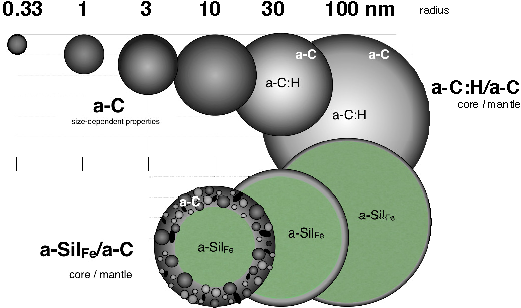
\includegraphics[width=150mm]{EPS/aa21686-13-fig1.pdf}
\caption{
In image from \cite{jones14} demonstrating a newly proposed model for dust composition, and showing that the dust story is far from concluded. a-C denotes amorphous carbon; a-C:H, hydrogenated amorphous carbon (HAC); a-Sil, amorphous silicon. The main point of the model is to propose that a mixture of amorphous carbon, amorphous silicates, and aromatized carbon is still supported but with an updated distribution of grain structures (some silicates may have amorphous carbon mantles) and updates to the typical size distributions. They propose a continuous distribution of grain structure from individual PAHs to amorphous carbon grains having an aromatized envelope, to silicates, to silicates with aromatic and/or amorphous carbon envelopes.
 }
\label{Jones Dust}
\end{center}
\end{figure}
\subsection{Carbonaceous Grains}
     As with silicates, it is well-established that carbonaceous material, primarily amorphous carbon, exists in the ISM \citep{aitken81,tielens87}. This is material commonly called ``soot" or the fuel we know on earth as coal.    Some non-amorphous carbonaceous material is also speculated to exist, such as graphite \citep{zhou06} or ``buckyonions" (concentric-shell-graphite) \citep{li08}. Even diamond has been proposed to exist in the ISM \citep{tielens87}, and has been discovered within meteorites thought to contain pre-solar material \citep{anders93}.
%\begin{figure}[htb]
%\centering
%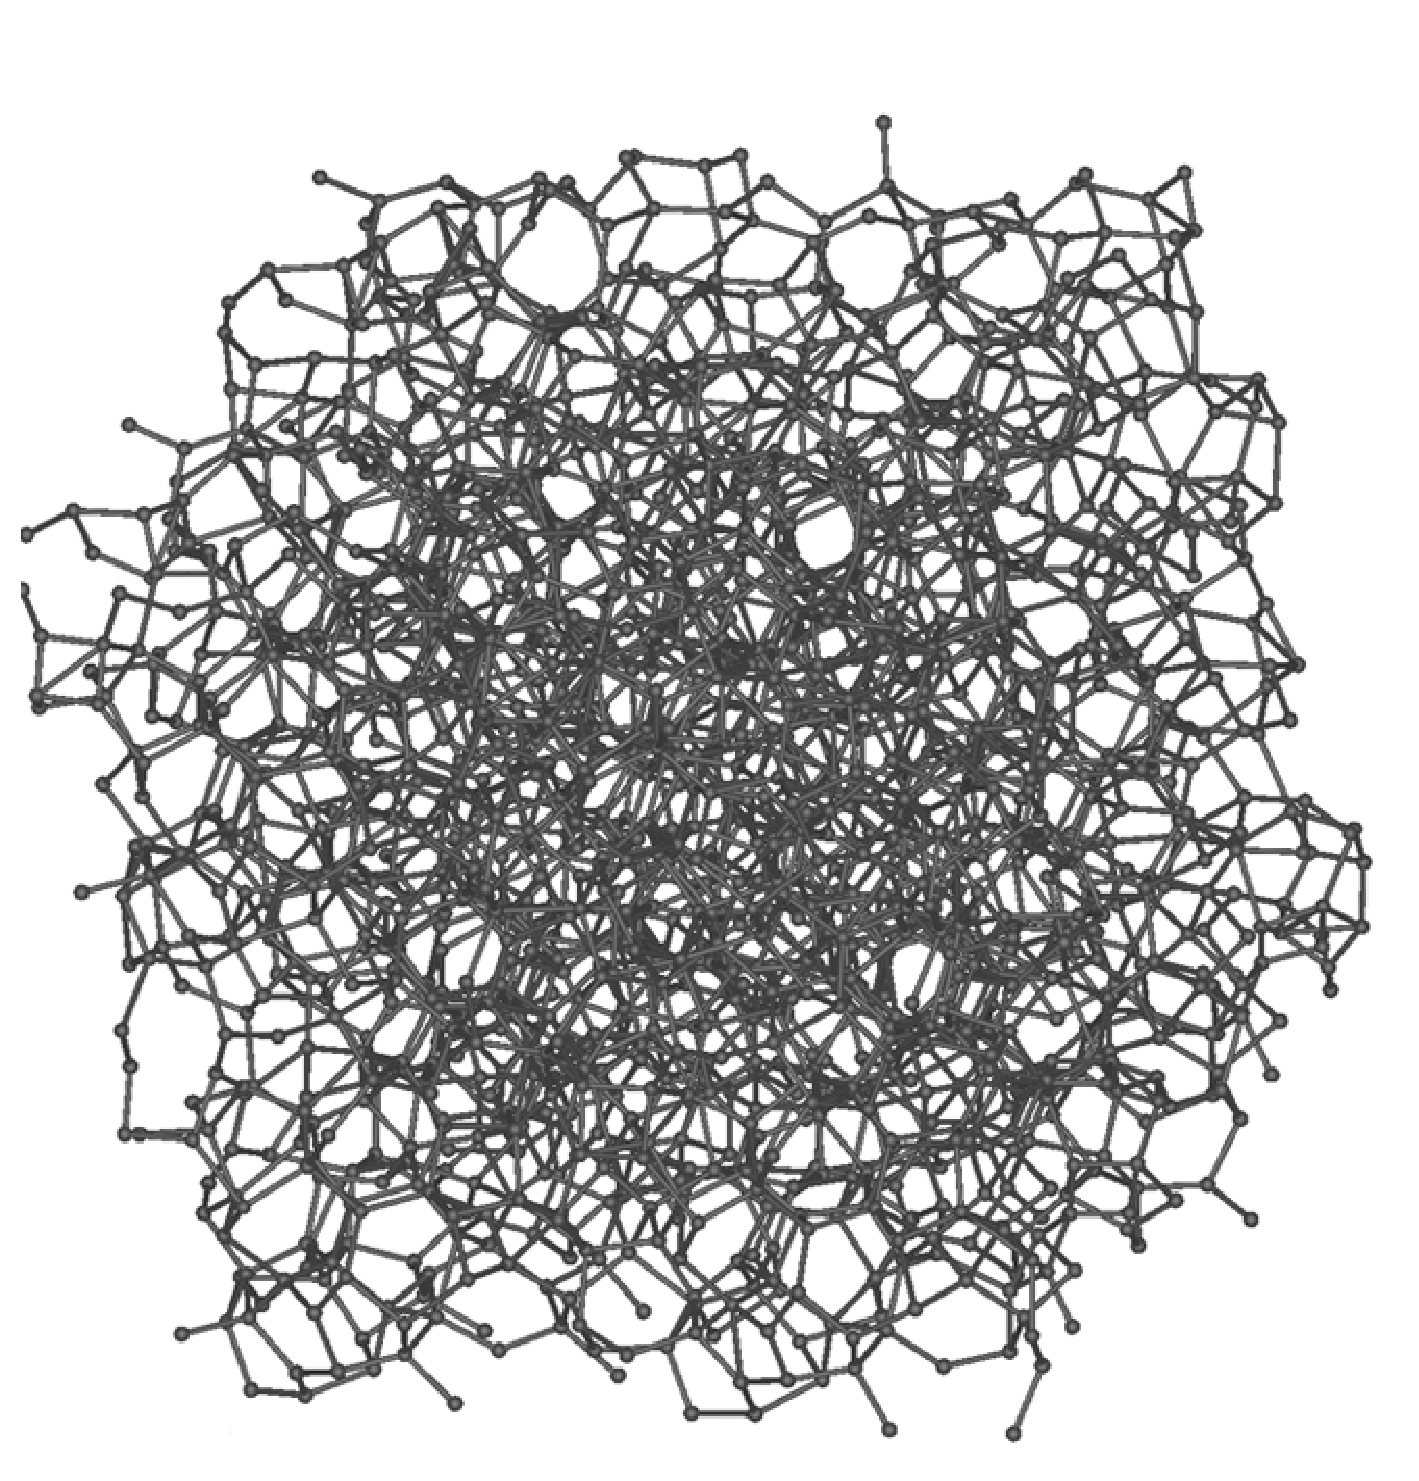
\includegraphics[width=100mm]{EPS/Amorphous_Carbon.pdf}
%\caption{
%Creative-commons image depicting the typical structure of amorphous carbon. The lack of an organized structure %leads to variations in the vibrational spectra.
% }
%\end{figure}
%%%%Ant Jones Figure???%%%
\subsection{The PAH Hypothesis}
\label{PAHhypothesis}
     Over the years since we have been studying interstellar material, the composition of dust has been debated heavily. 
     Within  the last 30 years, a popular hypothesis has arisen that a particular set of features of the interstellar medium SED between 3 and 12 microns, known as the ``Unidentified Infrared Bands" (UIRs), can be explained by the PAH family of molecules. The PAH interpretation was first proposed by \cite{allamandola85} and \cite{puget85}.
     With the appearance of high powered computers with an ability to perform rigorous calculations, many attempts have been made to simulate the expected emission from PAHs. Density functional theory (DFT) \citep{honenberg64} has become available as a tool for simulating molecular emission features using a quantum approach. DFT calculations has become a subfield of ISM astrophysics. Many attempts are being made to fit particular emission features of PAHs, and other molecular and grain species, to observed ISM features \citep{hammonds09,hirata99}.
     While it is difficult to reproduce the exact interstellar conditions in a laboratory setting, DFT simulations have yielded some evidence that the UIR bands can be explained as PAH vibrational emission features \citep{pathak12,ricca11,yu12}.

Some recent evidence by \cite{zhang14} has shown theoretically that mixtures of non-PAH carbonaceous and silicate spectra could also fit the theoretically calculated PAH emission features. However the PAH-UIR hypothesis is still widely supported \citep{tielens08,rastogi13}. The way that PAHs might be produced or evolve from other species is not understood however. Though there are efforts underway to model potential formation pathways. As far as the evolution of larger aromatics form smaller PAHs, there is one proposed pathway wherein a benzene could grow into a larger aromatic molecule such as naphthalene \citep{ghesquiere14}.

%%%Ahmit says Gillet is the first citation... GIllet 1973. But Allamandola 85 and leger 84 attributted them 戸PAHs。
%%% Or\cite{allamandola89}.???? %%%
%%%Existence of PAHs is being supported by DFT calculations matching observations. However there is some suggestion recently that other chemistries could produce the PAH bands, but this is not yet confirmed.
%%%Difficult to confirm PAH spectra in the laboratory, because difficult to get them into the gas phase as they would be in space.
%%%%Ahmit produced a thermal emission model ot the PAHs assuming some incident ISRF. See Pathak and Rastogi Temperature of the PAH will decrease in steps.
%%%PAHs are stable. The formation of the first ring may not be well understood, there is not experimental understanding of that step. The process of adding rings once the first is formed is more well understood. Pathway proposed where PAHs could serve as a substracte for the H2 formation. Adding of rings is well understood theoretically and experimentally. Another way to call the PAH bands is the aromatic infraared bands. Remember that PAH includes a wide class oof things. It is a molecule family. May be clusters of PAHs, inoized as well as neutral PAHs, and with chemical substitutions. PAH gives the whole family. It seems very clear that they would give the UIR bands.-Ahmit via Richter and Howard and Frank Klack
%%Don't forget to discuss the PAHs with respect to vibrational emission, and the way that multiple bands are produced from one UV excitation. 1E-6 second timescale for UV absorption to IR emissin -Ahmit. The fluorescene timescale is much longer. 
%%%Is there a referse process? Yes, for equal levels. Remember that a transition back to the ground state can also occur, producing a UV or visible photon.
%%%%Jones et al. 2014%%%%
\section{Galactic Microwave Foreground}

For astronomers wanting to study the microwave sky for cosmological purposes, there are foreground components which must be accounted for. These components arise from the simple reality that we are observing from inside the Milky Way. Our galaxy, and other galaxies, produces microwave emission which overlaps with frequencies important for the cosmic microwave background (CMB).

\subsection{Thermal (Vibrational) Dust Emission}
%%%Insert IRAS 100~$\mu$m or other plot showing the global dust emission%%%

In the optical, dust is interference. In the infrared, it is bright. The direct emission from dust, via thermal equilibrium vibrational modes, dominates in the far infrared (this is different from the stochastic heating and emission expected from very small grains, see Figure \ref{Transient heating of small grains}).

Assuming only emission by the vibrational modes, \cite{draine99} gives the power radiated per grain per frequency increment, $P_{\nu}d\nu$ as:

\begin{equation}
\label{spinpower}
P_\nu d\nu = 4\pi C_{abs}(\nu) B_\nu(T)
\end{equation}
where $B_{\nu}(T)$ is the Planck function per frequency, and $C_{abs}$ is the absorption cross-section at $\nu$.

\begin{figure}[htbp]
\begin{center}
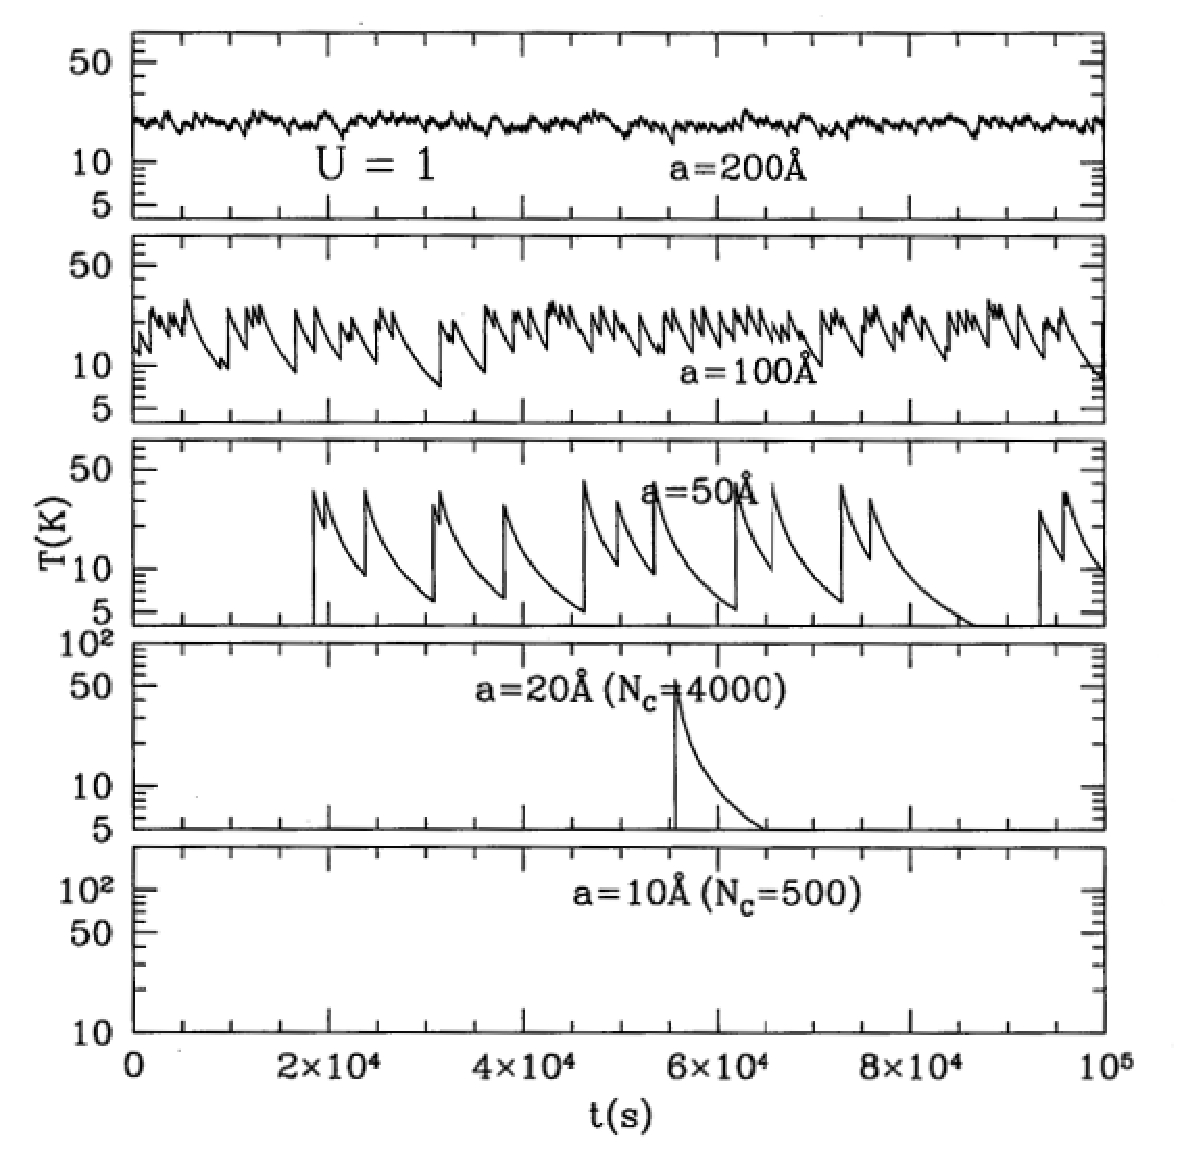
\includegraphics[width=150mm]{EPS/one-photon_heating.pdf}
\caption{
This diagram \cite{draine11} showing the heating and cool-down times of grains of various sizes. This example assumes a carbonaceous grain, and a radiation field equal to that of the solar neighborhood (U=1). Most importantly, note the lower plots: a grain of size 20 angstroms is heated and cooled very quickly. This is because when a grain is small enough, its heat capacity becomes close to the energy absorbed by an incident UV photon. They heat up very quickly; cool down very quickly. The top plot, for size 200 angstroms, shows that the grain temperature undergoes only small fluctuations.
 }
\label{Transient heating of small grains}
\end{center}
\end{figure}
%%%insert that figure describing grain temperature distributions%%
Though the exact shape of the dust SED for grains in thermal equilibrium varies across environments, and is not completely understood, it is well-approximated by a modified blackbody curve, as used in \cite{onaka99}. A modified blackbody simply means that a modification of the frequency dependence is applied to the Planck Law intensity, given below. For a blackbody, the intensity is proportional to the frequency, $\nu$ squared times the spectral radiance  per frequency, $B_\nu$ as a function of temperature, $T$.
\begin{equation}
I(\nu) \propto B_\nu{}(T)
\label{BBintensity}
\end{equation}
The intensity of a modified blackbody is given by the same proportionality above, but with a modification of the power law steepness. Thus the intensity of thermal dust emission, $I_d$ is given below. 
\begin{equation}
I_d(\nu) \propto \nu{}^{\beta{}_d}B_\nu{}(T_d)
\end{equation}
where $\beta$ is known as the ``emissivity index". The value of beta may vary, and the nature of these variations is a topic of intense discussion \citep{galliano11,juvela12}, but is commonly around 2.0 $\pm$ 0.5. The result of augmenting the blackbody with $\beta$ is such that a peaked continuum is still present, though the steepness of the SED is changed. 
%%%%insert citation for modified blackbody fitting and equation%%%
     This curve extends into the microwave realm, and if the amplitude is high enough, it may significantly overlap with other microwave sources. This is not a mysterious process, simply the microwave extremity of the well-studied infrared thermal emission process.
%%%%insert figure generated from Fred's code...show the modified BB fitting extended into the 30 GHz range%%
\subsection{Thermal Bremsstrahlung (Free-Free Emission)}
     Ionized gas in the galaxy will emit microwave radiation as the free electrons are accelerated. This becomes significant for foreground HII regions, and even more so for ultra-compact HII regions (UCHII). Free-free emission may be traced by H$\alpha$ surveys, as ionized hydrogen regions throughout the galaxy are thought to be the primary source of the galactic free-free foreground. Spectrally, free-free emission appears to follow a power-law distribution (related to the velocity distribution of the electrons in an ionized cloud). The typical value of the free-free spectral index, $\alpha$ is ~-0.13. However the exact separation of free-free emission from other galactic microwave foreground components is difficult, as the  frequency range 10 to 90 GHz overlaps with several galactic components \citep{wmap03b, leach08, planckXII}.
%\begin{center}
%\begin{equation}
%j_{ff,\nu}=\frac{8}{3}(\frac{2\pi}{3})^{1/2}g_{ff,i}\frac{e^6}{m^{2}_{e}c^{3}}
%(\frac{m_{e}}{kT})^{1/2}e^{\frac{-h\nu{}}{kT}}n_{e}Z^{2}_{i}n_{i}
%\end{equation}
%\end{center}
\begin{figure}[htb!]
\begin{center}
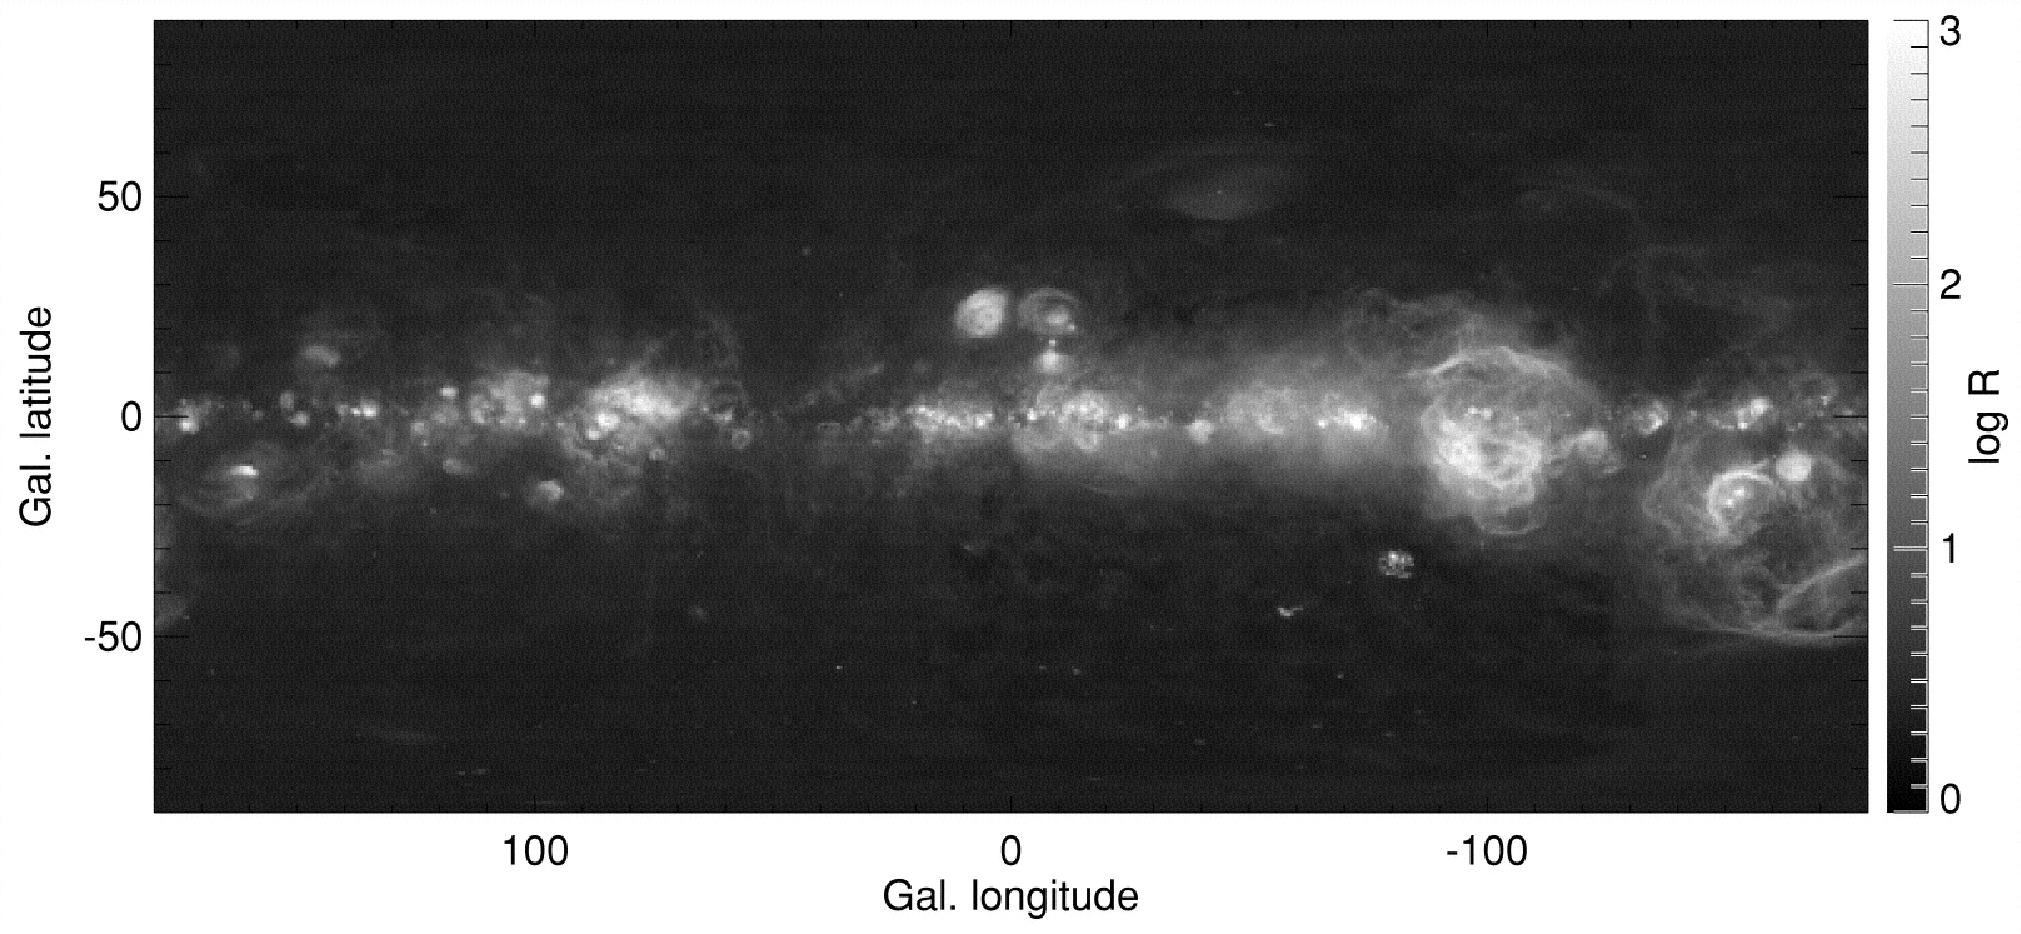
\includegraphics[width=150mm]{EPS/finkbeiner03_fg4_halpha.pdf}
\caption{
This is a template of H$\alpha$ emission for the galactic foreground, created by \cite{finkbeiner03}, derived from observation by the Wisconsin H-alpha Mapper (WHAM) \citep{wham98}, the Virginia Tech Spectral-Line Survey (VTSS) \citep{dennison98}, and the Southern H-Alpha Sky Survey Atlas (SHASSA) \citep{gaustad01}. The map is shown in galactic coordinates, and the greyscaling corresponds to the brightness in rayleighs ($1~R = 795.775\times10^6 [photons·m^{-2}·sr^{-1}]$). In their work, they describe that free-free emission should be well-traced by the amount of H$\alpha$, since free-free is produced from ionized gas clouds. However a free-free map is difficult to produce, since H$\alpha$ is an electronic emission feature and thus readily absorbed by intervening ISM. In order to derive the free-free contribution, the absorption of H$\alpha$ by dust must be corrected for. Estimating the free-free emission contribution is a critical step in order to isolate anomalous microwave emission.  
 }
\label{Dust}
\end{center}
\end{figure}

The free-free emission foreground has been studied extensively due to its relevance to (interference with) CMB investigations. In fact, attempts have been made to explain anomalous galactic foreground components via excess free-free emission \cite{kogut96}.

\subsection{Radial Bremsstrahlung (Synchrotron Emission)}

Driven by the Milky Way’s magnetic field, relativistically accelerated charged particles emit synchrotron radiation. The spectral shape of this radiation is very flat and predictable. Though it is not strongest in the microwave range, synchrotron emission is a significant foreground radiation field even at wavelengths around 30~GHz. 

When studying other microwave sources, we can control for synchrotron emission by looking at a less crowded frequency such as at 408~MHz. Figure 1.4 shows the radio survey by \cite{haslam82}, which is a useful tool for separating synchrotron emission from the AME, where synchrotron emission is the dominant component. From this lower frequency information the synchrotron flux density contribution,$S_{\rm sync}$, can be extrapolated to a target microwave frequency, $\nu$, using the following equation:

\begin{equation}
S_{\rm sync} = A_{\rm sync} \left( \frac{\nu}{{\rm GHz}}\right)^{\alpha}~
\label{synchrotron}
\end{equation}

This is the method used by \cite{planckXV} (hereafter, PCXV), where $A_{\rm sync}$ is the power law amplitude, $\alpha$ is the spectral index (having a typical value ~-3).
  
\begin{figure}[htb!]
\begin{center}
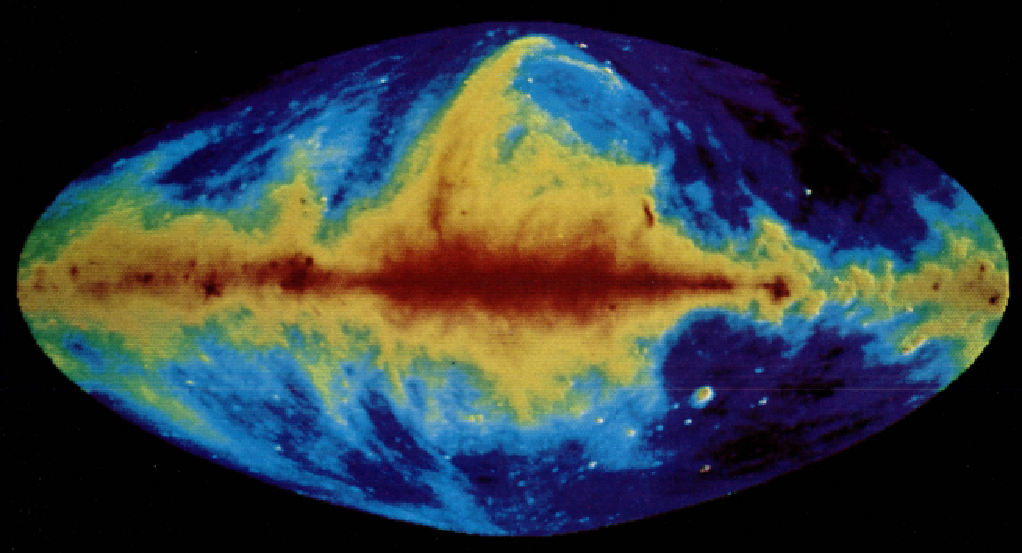
\includegraphics[width=150mm]{EPS/haslam403.pdf}
\caption{
408~MHz all-sky survey by \cite{haslam82}. The galactic foreground at this frequency is largely dominated by synchrotron emission. 
 }
\label{Dust}
\end{center}
\end{figure}

\section{Anomalous Microwave Emission}
%\label{sec:introduction:background}}
     Upon its first detection in early microwave surveys \citep{leitch97}, the AME or  ``Foreground X" \citep{deoliveiracosta02}, has been found to be a widespread feature of the microwave SED. That is, it appears over a very large portion of the sky. However its signature generally follows that of the galactic foreground of the Milky Way. The AME is almost certainly of galactic origin (we do not address the topic of AME in other galaxies, however a submm-mm excess has been noted been noted in the SMC, and attempts have been made to explain it as magnetic dipole emission, a similar process \citep{draine12}). Beyond the Milky Way-AME correlation however there is still much mystery, except that the most likely source of the AME is interstellar dust. \cite{kogut96,deoliveiracosta97,leitch98} showed that the AME correlates very well with dust, via the IRAS 100~$\mu$m surveys.
     Subsequently, \cite{ysard10b} compared the AME sky as revealed by WMAP \citep{wmap03a} to IRAS all-sky maps (see \ref{ysardcorrel}. They found a tighter correlation with dust at 12~$\mu$m than at 100~$\mu$m, implicating small dust (stochastically emitting dust). See Figure 1.2 for a description of the stochastic small grain emission, which was well-described by \cite{draine01}. 100~$\mu$m emission is produced by the larger, classically heated dust grains. More recently, using the cutting-edge Planck data, PCXV made a similar AME vs. IRAS comparison to that of \cite{ysard10a}, finding a similar result; IRAS 12~$\mu$m correlates more strongly with AME than IRAS 100~$\mu$m (see Figure 1.6).

\begin{figure}[htbp]
\begin{center}
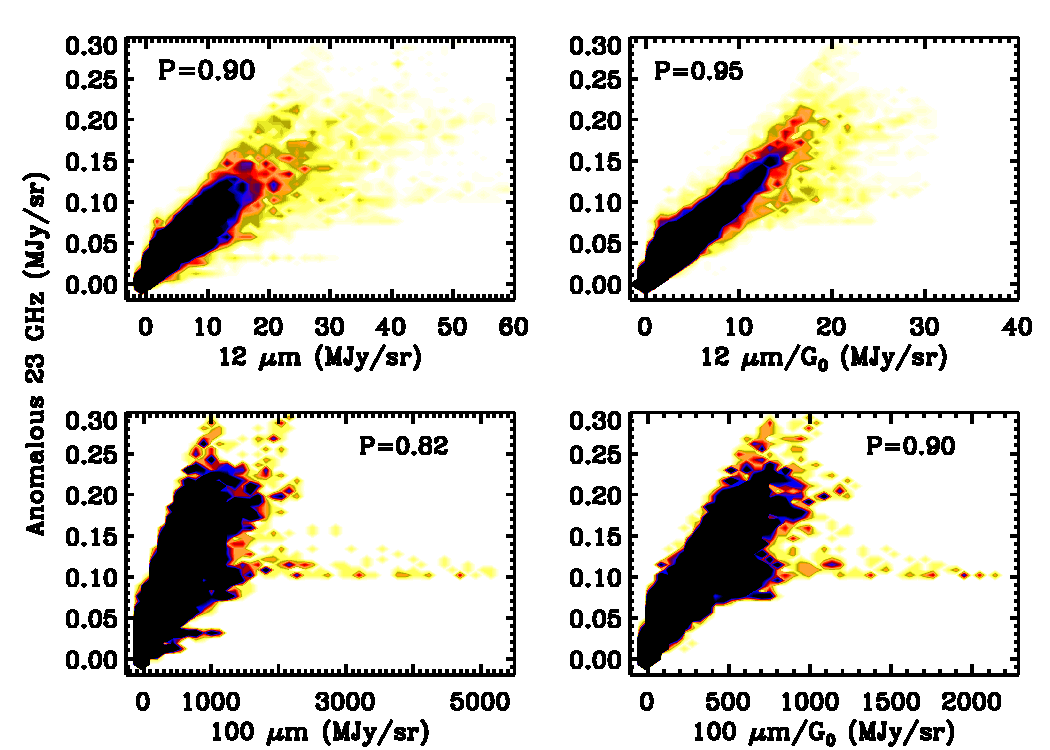
\includegraphics[width=150mm]{EPS/correl_ciel.pdf}
\caption{
A correlation test of AME (via WMAP) vs. thermal dust emission (via IRAS). Quoted from \cite{ysard10b}. The panels at left show simply the AME intensity at 23~GHz plotted against the IR intensity at 12~$\mu$m which traces mostly small grains (top), and 100~$\mu$m which traces mostly grains in thermal equilibrium (bottom). At right, the same data is plotted though with the IR intensities having been scaled by $G0$ value at each point. $G0$ is the intensity of the interstellar radiation field vs. that of the solar neighborhood. The correlation is stronger at 12~$\mu$m vs. 100~$\mu$m ($P=0.90$ vs. $0.82$). Both correlations improve slightly after scaling by $G0$.
 }
\label{ysardcorrel}
\end{center}
\end{figure}


\begin{figure}[tb]
\begin{center}
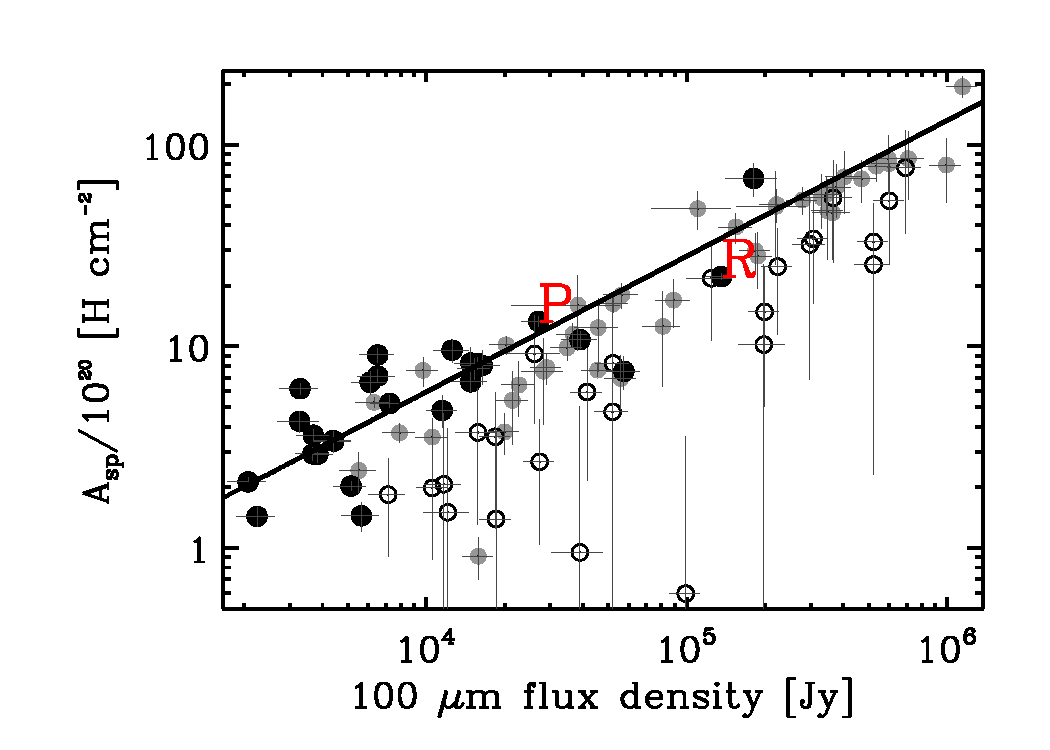
\includegraphics[width=0.45\textwidth]{EPS/fig18_1.pdf}
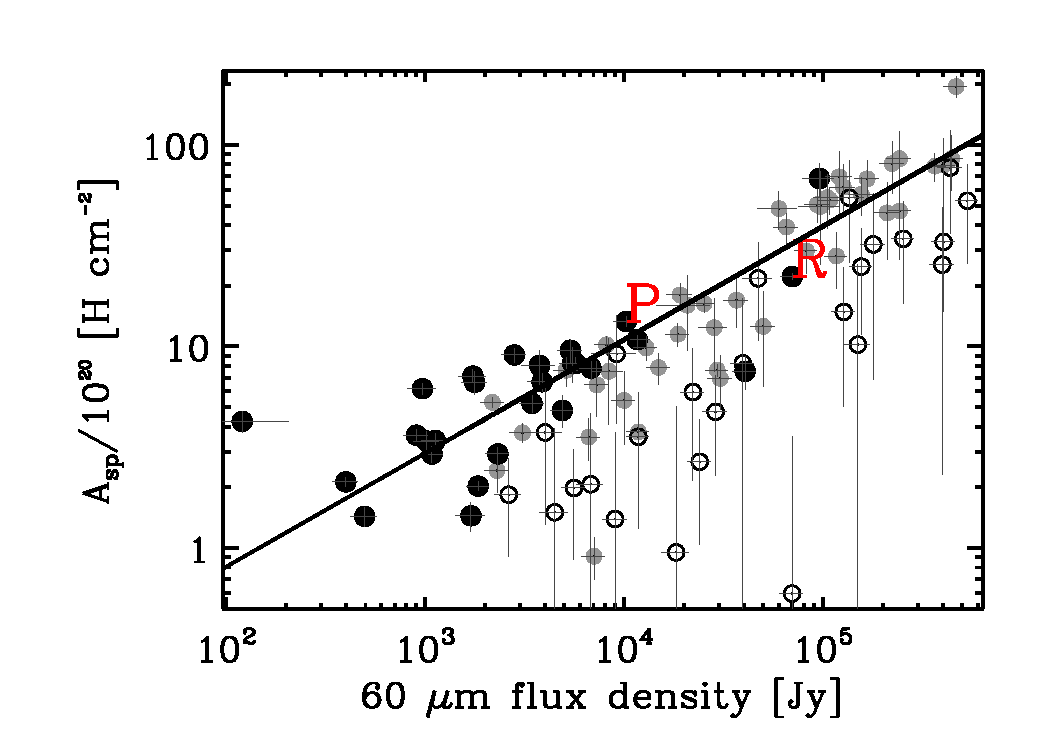
\includegraphics[width=0.45\textwidth]{EPS/fig18_2.pdf}
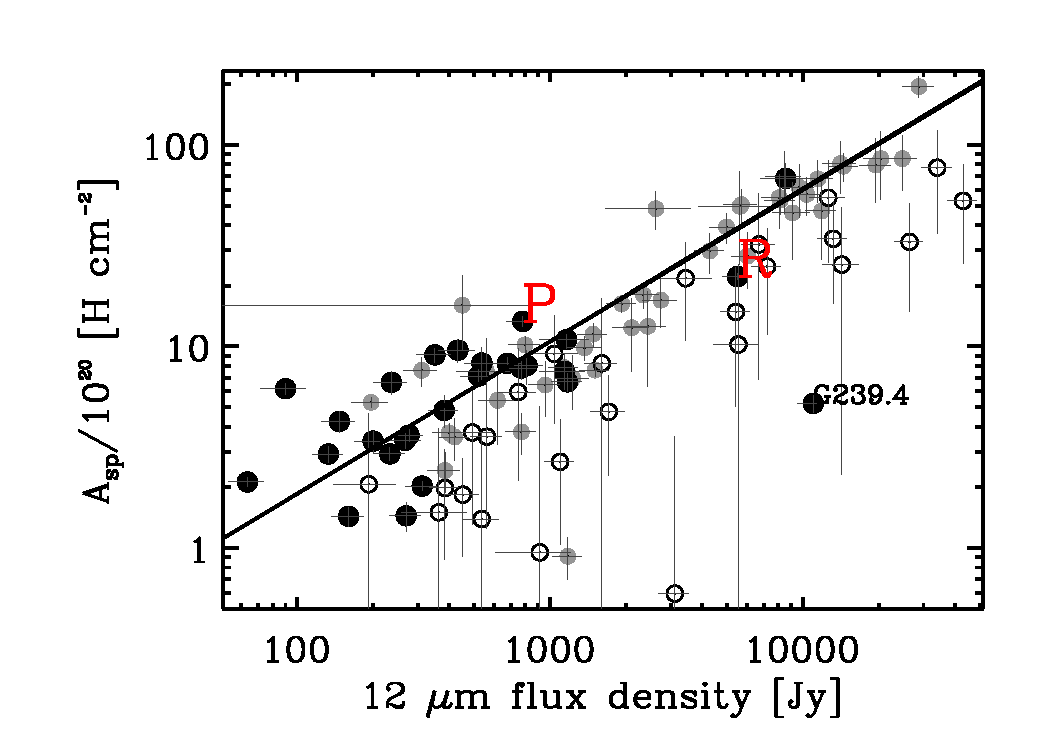
\includegraphics[width=0.45\textwidth]{EPS/fig18_3.pdf}
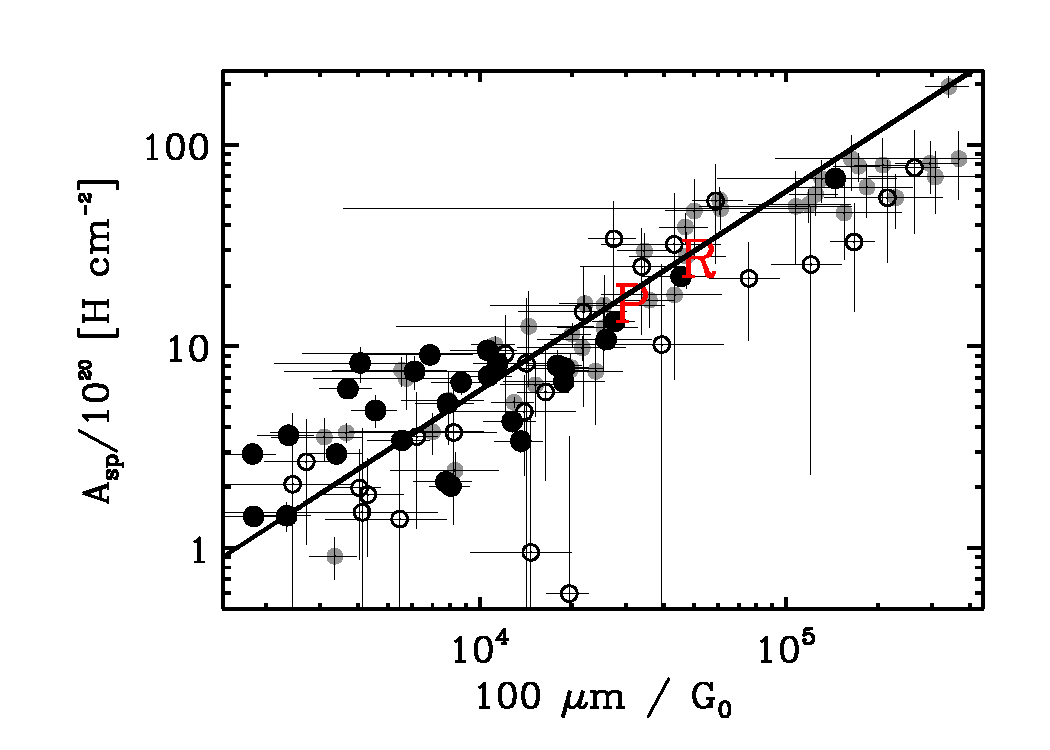
\includegraphics[width=0.45\textwidth]{EPS/fig18_4.pdf}
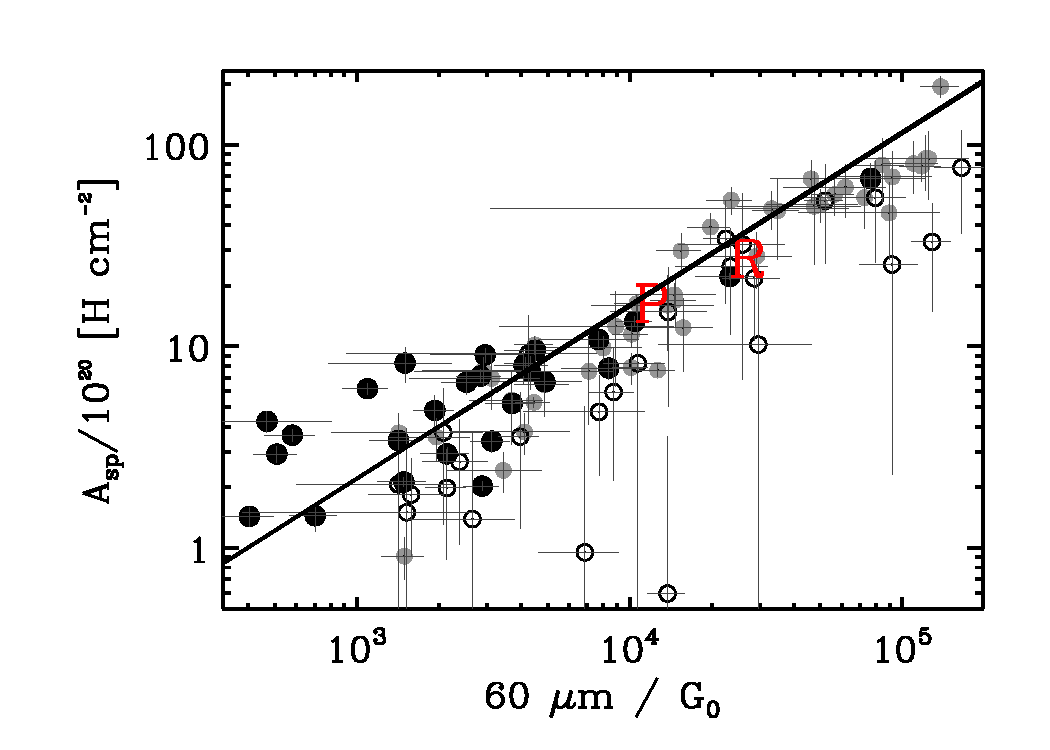
\includegraphics[width=0.45\textwidth]{EPS/fig18_5.pdf}
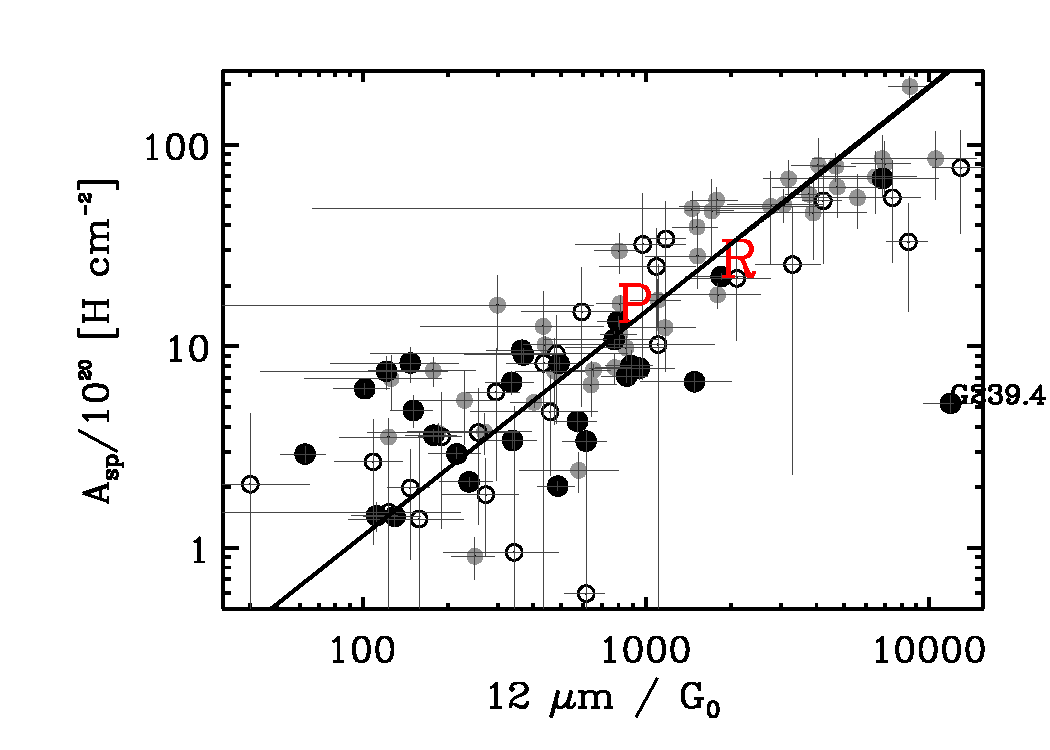
\includegraphics[width=0.45\textwidth]{EPS/fig18_6.pdf}
\caption{Dust Correlations from \cite{planckXV}, based primarily on Planck LFI \citep{lfi14ii} microwave data and IRAS IR data. The top 3 plots show the AME amplitude (which is \textit{``roughly equivalent to the column density of spinning dust, assuming there is no shift in peak frequency"}, according to \cite{planckXV}) vs. the total flux density [Jy] at the IRAS IR wavelengths of 12, 60, and 100~$\mu$m. Their flux densities were summed over a 1$\degree$ radius circular aperture (after smoothing the data to 1$\degree$ resolution}
\label{planckcorrel}
\end{center}
\end{figure}
     We once thought emission in the 10 to 90~GHz frequency domain was sourced by a combination of the cosmic microwave background (CMB), free-free emission, and synchrotron radiation. The RING5M CMB experiment in the 1990s cast some doubt on this explanation when excess microwave flux was detected near the north celestial pole by \cite{leitch98}. They describe that although the CMB contributed 90\% of their extracted signal: \textit{``Our 14.5 GHz observations of the NCP have also resulted in the detection of an anomalous component of Galactic emission [...] a cautionary tale for future CMBR experiments."}
     AME has been shown to take the shape of a ``sub-millimeter bump”, an excess over the expected free-free and synchrotron emission. The peak of this bump is typically around 30~GHz (PCXV). Given the typical spectrum and its peak frequency, PAHs have been proposed as a likely carrier of the AME. PAHs which are rapidly spinning and which have a permanent electric dipole should produce microwave emission. However there is a secondary explanation, the possibility of a contribution from magnetic dipole emission (these will be explained in more detail in the following sections). These two mechanisms are not mutually exclusive, and the spectrum of magnetic dipole emission has also been theoretically determined by \cite{draine99}. They report that this emission should overlap with spinning dust emission.
     As the microwave sky was revealed in more and more detail, the anomaly became more of an unexplained galactic foreground component. AME was detected not only towards the NCP, but in several prominent regions which were not expected to show bright microwave emission. The $\rho$ Ophiuchi molecular cloud is one of these \citep{casassus08}. 
     This microwave foreground has been studied extensively since then. AME has been correlated with thermal dust emission, leading to the suggestion that AME is electric dipole emission from spinning dust \citep{draine98b}. All-sky comparisons between WMAP and IRAS maps further support the correlation with the Milky Way, and with dust. The 100 micron (3~THz) IRAS map correlates well with the AME, and more interestingly the 25 micron maps shows an even tighter correlation \citep{ysard10a}. One implication of such an observation is that the AME is likely carried by small grains rather than larger grains.
\subsection{Spinning Dust Emission}
\label{spinningdust}
     One of two prevailing explanations for the AME, has been electric dipole emission from small spinning dust grains. Rotational emission from molecules is of course well-modelled and observed, as in the case of CO emission. Rotational excitation is by no means rare; it is simply another fundamental mode by which molecules move and interact. The mystery is which molecules could produce the shape and intensity of the AME spectrum?
     Grains or molecules having a permanent electric dipole,  rotationally should emit electric dipole radiation. This may be due to ``spillover" from the photo-excited vibrational modes into the rotational modes or, direct rotational excitation by collisions, such as with atoms or ions. The observed intensity in this model is proportional to the dipole moment magnitude (length of the dipole separation and magnitude of the charge) of the spinning molecule, and the column density of the spinning grains (number of oscillators) along the line of sight. 
     The physics involved are very simple, and the model was first proposed by \cite{draine98a}. They have shown that small spinning dust grains or large molecules with a permanent electric dipole,  can reproduce the shape of the anomalous continuum SED. If the torque applied to the grains is strong enough, the ``amplitude" of the AME feature may also be reproduced. Using a rough spherical-grain assumption for the sake of demonstration, the following equation gives the power emitted per spinning grain, $P$, having an electric dipole of magnitude $\mu$, spinning at a frequency of $\omega$. $c$ is the speed of light. 
\begin{center}
\begin{equation}
P = {4\over9} {\mu^2\omega^4\over c^3}
\label{eq:Pspin}
\end{equation}
\end{center}
     If this is the power per grain, then an increased abundance of rotating grains would obviously result in more observed AME flux (since the number of oscillators is increasing).
     \cite{draine98a} then gives the expected rotational frequency $\omega$ at a temperature $T=100~K$ as follows, where $a$ is the grain size, and $\xi$ represents the deviation from a spherical moment of intertia:
\begin{equation}
{\omega_T\over 2\pi} = 
\langle\nu^2\rangle^{1/2}
\approx 5.60\times 10^9 a_{-7}^{-5/2}\xi^{-1/2}T_2^{1/2}~~~{\rm Hz}~,
\label{eq:nurms}
\end{equation}
%%%Equation from Draine 1998%%%
%\begin{center}
%\begin{equation}
%\label{spinningdust}
%\mu^2 = 
%[(4.8)^2\left({a_x\over a}\right)^2 \langle Z^2\rangle + 
%(9.3)^2a_{-7}]a_{-7}^2 (debye)^2 ~~~.
%\end{equation}
     From equation \ref{eq:nurms}, we can note that the peak AME frequency should depend on the grain size. We can use this to make a rough estimate of the oscillator's size: starting with the average peak AME frequency, around 30~GHz, a dust temperature of about 100~K, and a simple spherical moment of inertia, Equation 1.4.2 implies a spinning grain size on the order of 10~nm. \citep{draine98b}. This suggests extremely small dust particles. The typical size of PAHs is in the nanometer range (though PAHs can take on a wide range of shapes). This is a small clue which leaves further evidence heavily desired, in order to confirm or deny PAHs (or PAH-based species) as an AME carrier. Several possible PAH-family AME carriers have been proposed, such as naphthalene. Naphthalene is mentioned above as having a possible formation pathway in the ISM. The chemical substitutions inside naphthalene, deviating from the ``pure" PAH structure would give it a dipole moment. Detection of naphthalene features in a the prominent AME region, the Perseus Molecular Cloud, has been reported by \cite{iglesiasgroth08}.
%%%%Need to discuss ways that PAHs could have a dipole moment. Size alone doesn:t matter, as in the case of corronene vs. corranulene.
%%%% Chemical modifications could be one scenario.....- Hudgins et al.
%%%%%%%% One example is HCN type things. Or ''PAHNs". This has not been demonstrated to be plausible experimentally, it is just a theoretical suggestion.
%%%% Could be structural moments, like the 3D shape of corranulaene. 
     Many subsequent papers have been published since Draine \& Lazarian's (1998) calculations were presented, further supporting the spinning grain hypothesis and refining the theory, as in the case of \cite{hoang10}, wherein grain rotation not about an axis of symmetry is examined. These papers show that even after accounting for variations of grain shape, the spinning-dust hypothesis remains plausible. However the chemical composition of these supposedly spinning grains remains a mystery.
     Early models only implicate the rough size of the grain, and the models allow for some variation of the shape. An exact chemical species or class of grain types, or a prevailing mixture has yet to be strongly observed in AME regions or predicted by models.

\subsection{Magnetic Dust}
     Magnetic dipole emission has also been proposed as an emission mechanism for this same frequency range by \cite{draine99}. Thermal fluctuations in grains that have magnetic inclusions should produce a spectrum which could overlap with the spinning dust models, and observed AME frequencies. This is described in Figure 1.7.
%They give the following equation to describe to power radiated via magnetic dipole emission from dust:
%\begin{equation}
%\frac{j_{\nu{}}}{n_{\H{}}}=\frac{n_{gr}V}{n_{H}}\frac{4\pi{}h\nu{}^{4}}{c^{3}}\frac{1}{\exp{(h\nu/kT)-1}}\frac{9\mu{}_{2}}{(\mu{}_{1+2})^{2}+\mu{}_{2}^{2}}
%\end{equation}
\begin{figure}[htb!]
\begin{center}
\label{magneticdust}
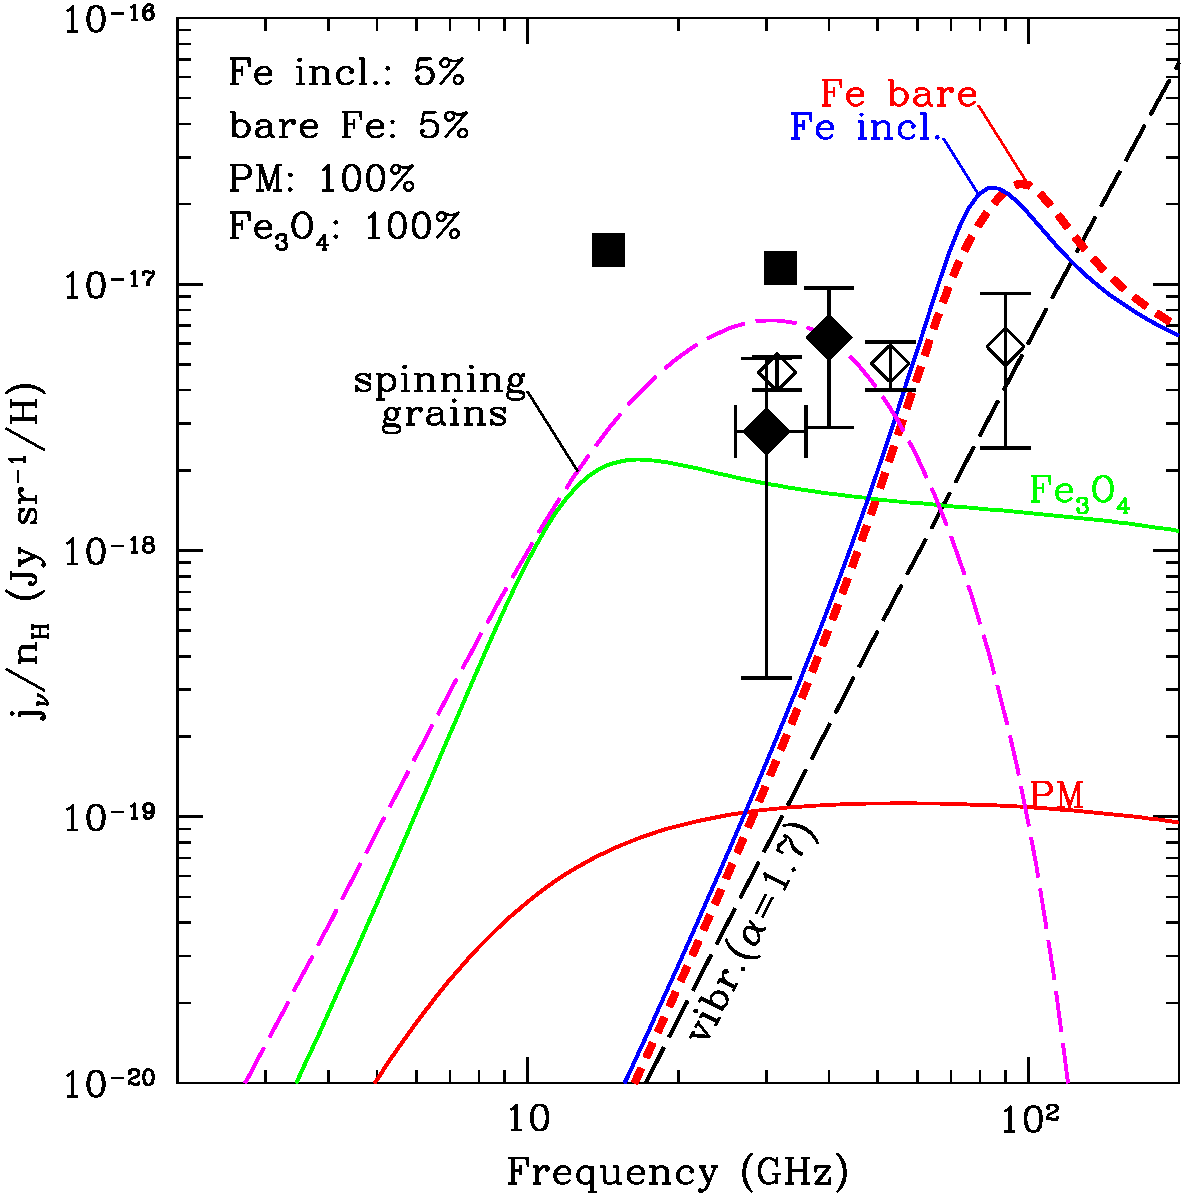
\includegraphics[width=100mm]{EPS/draine99_fig7.pdf}
\caption{From \cite{draine99}, this plot describes an early model of the ''anomalous" modes of dust emission. It is included here to give some perspective on the exptected relative contributions of thermal dust (``vibr., $(\alpha = 1.7)$", long dashed black), spinning dust, and magnetic dust. Squares and diamonds are observational points from early CMB observations. The axes are frequency in GHz (note the peak of spinning dust at ~30~GHz, and how this peak overlaps with all plotted emission components) against intensity per hydrogen column density (Jy $sr^{-1}$/H).They plot the electric dipole (``spinning grains" contribution (magenta long-dashed) along with the various expected magnetic dipole contributions from bulk iron (``Fe bare", short red dashed), grains with iron inclusions (``Fe incl.", blue solid), iron oxides ($Fe_{3}O_{4}$, green solid) and paramagnetic grains (``PM", red solid).} 
\end{center}
\end{figure}
     There a few regions such as $\rho$~Ophiuchi that are still thought to be dominated by spinning dust \cite{casassus08}. Studies of the AME and diffuse galactic emission done by \cite{planckXVii} show some evidence for an additional blackbody microwave component which could be caused by magnetic dust in the diffuse sky.  Whether or not their result also applies to galactic clouds is unclear. \cite{draine99} describes the potential contribution of magnetic dust in the following way: \textit{``one cannot exclude the possibility that magnetic grains make an appreciable contribution to the emission in this frequency range."}

\section{Motivation for Understanding the Anomalous Foreground}
     Perhaps a primary factor for why the AME was ever noticed, and why it is worth understanding, is its interference with non-ISM topics. \cite{leitch97} features a warning to other researchers upon their detection of the AME: \textit{``The detection of such a component suggests that we should be cautious in any assumptions made regarding foregrounds when designing experiments to map the microwave background radiation.”} More recently, it was shown via 
data by \cite{macellari11} that the AME is a dominant component of the microwave foreground at low galactic latitudes. Thus, getting a full picture of the CMB's anisotropies will be difficult without considering the intervening material that is the Milky Way.
     In a similar way, gravitational wave astronomy may be somewhat hindered by the less understood emission mechanisms of interstellar dust. The second-generation of the Background Imaging of Cosmic Extragalactic Polarization observations (BICEP2) reported a detection of a B-mode polarization signal in the CMB in \cite{ade14}.
     Follow up studies have proposed that this initial detection may in fact be confused with the galactic microwave foreground, in the form of magnetic dipole emission from dust \citep{liu14}. However it is still unclear what the contribution from dust could be, as the polarization data is still being reviewed.  In any case, the B-mode polarization due to inflation in the early universe cannot be confirmed without constraining a possible contribution from dust \citep{flauger14,mortonson14}.
     From the ISM perspective too, the AME's origin is important beyond simply its possible confusion with cosmological data. The source of AME has implications for the ISM itself. Spinning dust may be another piece of the ``ISM Interaction Puzzle”. If the AME is linked strongly to spinning dust, or to magnetic dust, it could be used as a probe for ISM conditions.
     Confirmed spinning dust emission could imply possible presence of some certain chemistries (perhaps PAHs, or other small dust having an electric dipole.) For example, confirming that AME = spinning dust, would allow us to probe galactic environments in the case that corresponding vibrational modes of those spinning molecules are found to be missing. If AME is carried by very small dust grains or by PAHs, then microwave emission could be used to trace these molecules more clearly even if their vibrational emission is being obscured along the line of sight. \cite{tibbs14} attempt to derive small grain properties within molecular cores assuming that the AME there is from spinning dust, as an early example of using AME to understand the ISM. 
     Confirmed magnetic dust emission as part of the AME could help to constrain the composition of dust. As \cite{draine99} has shown that grains with Fe inclusions could produce this emission, magnetic dust emission may help determine the abundance of ferromagnetic dust. The search for magnetic dust emission may also be a potential test of the model put forth by \cite{jones14} (see Figure \ref{Jones Dust}) wherein some silicate grains may have iron inclusions.
\clearpage

\section{Contents}  
  In Chapter \ref{chap:Introduction} we have described the basic issues of ISM and dust research, and highlighted the importance of understanding the anomalous microwave emission foreground. The AME is very likely to originate from dust. Spinning dust emission and magnetic dipole emission from dust are the leading explanations.  
  In Chapter \ref{chap:Data} we give an introduction to the data sources used for this work. As this is a study based only on space-telescope data, there are no specific observational techniques to describe. Rather, the relative characteristics of each of the 13 all-sky photometric maps used are discussed. We describe the importance of each instrument, and highlight the advantages of using the new MIR surveys by AKARI/IRC and the newly released  FIR surveys by AKARI/FIS. Most important to this work is the combination of AKARI/IRC and Planck/HFI, and this is shown by the relative response functions of each band.
  The data processing is described in Section 2.4. The major objective of the data processing method is to create a set of maps, ranging the full thermal dust SED, at an identical pixel size and smoothing scale.  We then describe how information regarding the dust at each pixel is inferred, such as the temperature, emissivity index, and relative sub-micron dust abundance. 
  In Chapter ref{chap:Analysis} we describe how the dust properties extracted from the average dust SEDs from each of the AME regions is compared. Plots demonstrate the relative strength of the correlations of each photometric band's average intensity vs the AME amplitude for each ROI. We also update a previous work regarding the ratio of the AKARI/IRC 9~$\mu$m band to the 18~$\mu$m band intensity vs. the significance of spinning dust reported by PCXV.
  In Chapter ref{chap:Discussion} we comment more deeply on the methods used, and discuss possible interpretations of the analysis in Chapter 3. We discuss the lack of strong support for a clear PAH-AME relationship, and present pathways for further investigation.
  A summary is given in Chapter 5.
